

\documentclass[10pt,twocolumn,letterpaper]{article}

%%%%%%%%% PAPER TYPE  - PLEASE UPDATE FOR FINAL VERSION
% \usepackage[review]{cvpr}      % To produce the REVIEW version
\usepackage{cvpr}              % To produce the CAMERA-READY version
%\usepackage[pagenumbers]{cvpr} % To force page numbers, e.g. for an arXiv version

% Include other packages here, before hyperref.
\usepackage{graphicx}
\usepackage{amsmath}
\usepackage{amssymb}
\usepackage{booktabs}
\usepackage[shortlabels]{enumitem}


% It is strongly recommended to use hyperref, especially for the review version.
% hyperref with option pagebackref eases the reviewers' job.
% Please disable hyperref *only* if you encounter grave issues, e.g. with the
% file validation for the camera-ready version.
%
% If you comment hyperref and then uncomment it, you should delete
% ReviewTempalte.aux before re-running LaTeX.
% (Or just hit 'q' on the first LaTeX run, let it finish, and you
%  should be clear).
\usepackage[pagebackref,breaklinks,colorlinks]{hyperref}


% Support for easy cross-referencing
\usepackage[capitalize]{cleveref}
\crefname{section}{Sec.}{Secs.}
\Crefname{section}{Section}{Sections}
\Crefname{table}{Table}{Tables}
\crefname{table}{Tab.}{Tabs.}


%%%%%%%%% PAPER ID  - PLEASE UPDATE
\def\cvprPaperID{*****} % *** Enter the CVPR Paper ID here
\def\confName{CVPR}
\def\confYear{2023}


\begin{document}

%%%%%%%%% TITLE - PLEASE UPDATE
\title{NTIRE 2023 Efficient SR Challenge Factsheet \\
	LGTT: Local-Global Term Transformer for SR}

\author{Jinchen Zhu, Jinpeng Shi, Hui Li, Shizhuang Weng\\
Anhui university\\
Anhui,China\\
{\tt\small jinchen.Z@outlook.com,jinpeeeng.s@gmail.com}
% For a paper whose authors are all at the same institution,
% omit the following lines up until the closing ``}''.
% Additional authors and addresses can be added with ``\and'',
% just like the second author.
% To save space, use either the email address or home page, not both
}
\maketitle

\begin{figure*}[htp]
	\centering
	\centering
	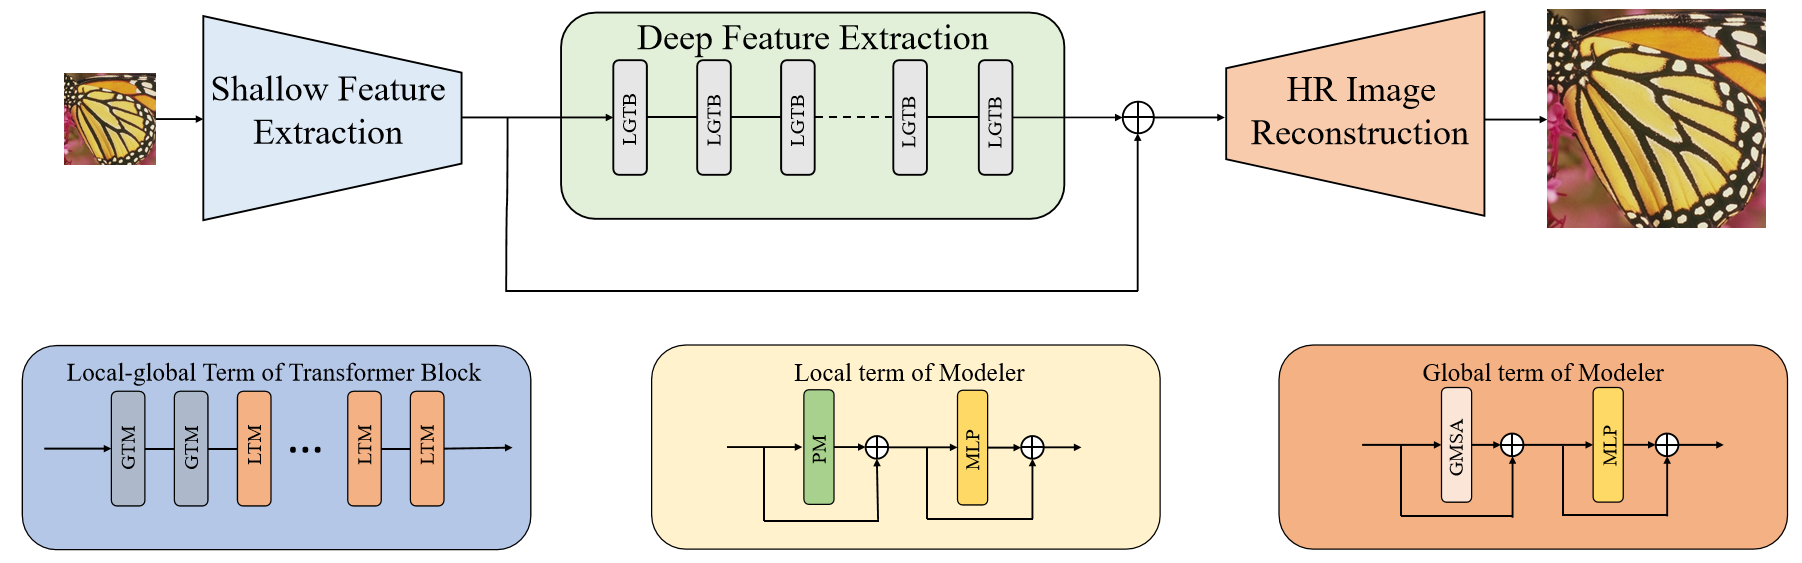
\includegraphics[width=1\linewidth]{Image/Arch}
	\label{trans_sparse}%文中引用该图片代号
	\caption{Illustration of the LGTT.
	}
	\label{arch}
\end{figure*}
\begin{figure*}[htp]
	\centering
	\centering
	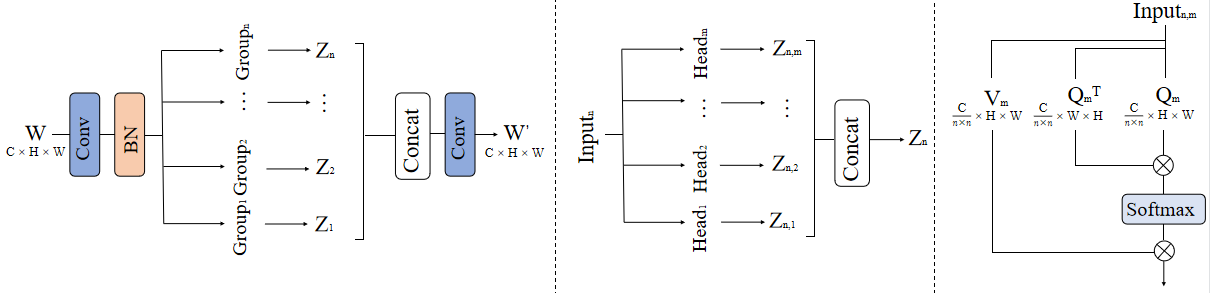
\includegraphics[width=1\linewidth]{Image/multi_sa}
	\label{trans_sparse}%文中引用该图片代号
	\caption {Illustration of our multi-groups multi-heads SA mechanism, updated on the basis of \cite{ESWT}. The left figure shows
	the multi-groups mechanism, which divides the groups according to the number of different windows of the input, as a way
	to increase the speed. The middle figure shows the multi-heads mechanism, where each group can have n heads in it, while
	computing self-attention. The right figure shows the calculation of SA on a head.
	}
	\label{GMSA}
\end{figure*}

\section{Team details}

\newcommand{\github}[1]{\href{https://github.com/#1/}{github.com/#1}}

\begin{itemize}
	\item Team name: \textbf{FRL Team 0}                                  
	\item Team leader name: \textbf{Jinchen Zhu}                          
	\item Team leader address, phone number, and email:
	\begin{itemize}
		\item address: \textbf{Anhui University, Hefei, China}
		\item phone number: \textbf{+86 188 5507 6340}
		\item email: \textbf{jinchen.Z@outlook.com}
	\end{itemize}
	\item Rest of the team members: \textbf{Jinpeng Shi (advisor)}, \textbf{Shizhuang Weng (advisor)} and  \textbf{Hui Li}
	\item Team website URL (if any): \\ \github{Fried-Rice-Lab/FriedRiceLab}                   
	\item Affiliation: \textbf{Anhui University}
	\item Affiliation of the team and/or team members with NTIRE 2023 sponsors (check the workshop website): \textbf{N/A}
	\item User names and entries on the NTIRE 2023 Codalab competitions (development/validation and testing phases):
	\begin{itemize}
		\item user name: \textbf{Jinchen.Z}
		\item development entries: \textbf{7}
		\item validation entries: \textbf{8}
	\end{itemize}
	\item Best scoring entries of the team during development/validation phase:
	\begin{table}[h]
		\centering
		\resizebox{\linewidth}{!}{
			\begin{tabular}{|c|c|c|c|c|c|}
				\hline
				PSNR&SSIM&Runtime&Params&Extra Data\\
				29.00 (21) 
				&0.83 (20)& 0.07 (20)& 118243.00 (5) &1.00 (1)\\
				\hline
			\end{tabular}
		}
	\end{table}
	\item Link to the codes/executables of the solution(s): \\ \github{Jinchen2028/NTIRE2023\_ESR}
\end{itemize}

\textbf{Fried Rice Lab} (FRL) is organized by students from Anhui University who are interested in image restoration. FRL is dedicated to proposing clean and efficient image restoration solutions and contributing to the image restoration open source community. \textbf{FRL Team 01}, lead by Jinchen Zhu and advised by Jinpeng Shi, was among the teams that FRL sent to compete in the NTIRE 2023 ESR competition, with \textit{Someone (replace if any)} completing the roster.

\section{Method details}
\noindent{\bf General method description}
There is already a lot of work trying to reduce the complexity of SA, including \cite{performer,sparsetrans,reformer}. Our goal is to reduce the complexity of transformer for SR and maintain its performance,so we propose Local-Global Term Transformer (LGTT) for SR , not every group needs self attention. The overall architecture is shown in the Figure \ref{arch}. In order to establish long-term dependencies efficiently, a pair of SAs is reserved in each group as a Global-term Modeler and using the striped window mechanism\cite{ESWT}, avoiding redundant operations. we improve BWSA by adding multi-groups and multi-heads mechanisms to improve computational efficiency,i.e., multi-head group WSA (GMSA), as shown in the Figure \ref{GMSA}. In the rest of the blocks we propose efficient pixel mixer (PM) modules to without computational cost and can efficiently model short distance dependencies as a Local-term modeler. which will be mentioned later about the PM module.
\\ \hspace*{\fill} \\
\noindent{\bf Pixel Mixer}
\label{PM}
We propose the pixel mixer module without parameters and computational complexity to create short-distance dependencies in each input Token. The PM module first divides the feature channels into five groups equally and moves the edge feature points to the opposite side in the order of left, right, top, and bottom for the first four groups. By inputting an intermediate feature of H $\times$ W $\times$ C, the PM module enables each input window in SA to obtain different local information according to other channels by linking the edge feature points with the opposite edge feature points respectively, so that each feature point can be fully utilized and the perceptual field of the later module can be increased.

\section{Training strategy}
We use DF2K (DIV2K\cite{DIV2K}, Flickr2K\cite{EDSR})and LSDIR for datasets. and propose that the channel input is set to 30, the data augmentation method with $90^\circ$, $180^\circ$, $270^\circ$ random rotation and horizontal flip is used for training, the batchsize is set to 128, and the input patch size of LR is $64\times64$.Trained using Adam optimizer\cite{Adam} with $\beta_1$ = 0.9, $\beta_2$ = 0.999. The initialized learning rate is $5\times10^{-4}$ and decays to $1\times10^{-6}$ with the cosine learning rate. The model is optimized using the loss function of $L_1$ for a total of $1\times10^6$ iterations. Model training was performed using Pytorch\cite{pytorch} on two NVIDIA V100 32G GPUs.

\section{Experimental results}
We test our model on the DIV2K and LSDIR test sets, and the experiments are performed on a V100, using the official code. The results is shown in Table \ref{test}.
\begin{table}[h]
	\centering
	\resizebox{\linewidth}{!}{
		\begin{tabular}{|c|c|c|c|c|c|}
			\specialrule{0em}{1pt}{0pt}
			\hline
			PSNR&SSIM&Params[K]&FLOPs[G]&Conv&Average Runtime[ms]\\
			\hline
			27.02 (21)&0.81 (17)&115 (3)&7.38&58&0.08 (18)\\
			\hline
		\end{tabular}}
	\caption{ Result of DIV2K and LSDIR test sets}
	\label{test}
	
\end{table}


%%%%%%%%% REFERENCES
{\small
\bibliographystyle{ieee_fullname}
\bibliography{egbib}
}

\end{document}
